\textbf{2. Representación y ajuste de las gráficas}

\vspace{20px}

Para representar las dos gráficas pedidas, se eliminan las galaxias que tienen desplazamiento espectral negativo.

Seguidamente, se ajustan los datos a una recta que pase por el origen. Las gráficas, con el valor de pendiente obtenido,
se pueden ver a continuación.

\vspace{20px}

\begin{center}
    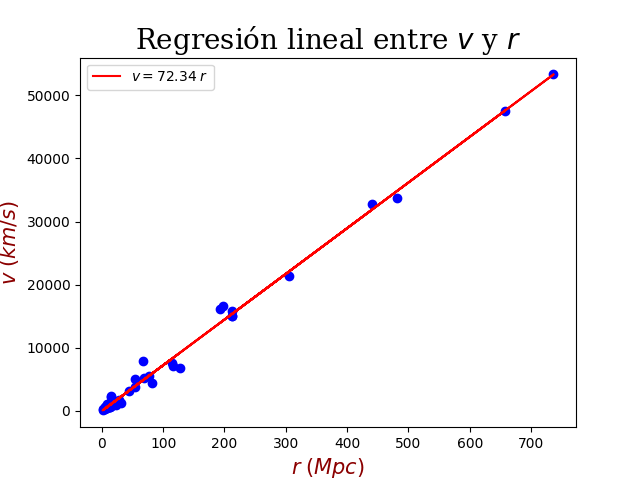
\includegraphics[scale=0.45]{files/plot1}
\end{center}

\vspace{20px}

\begin{center}
    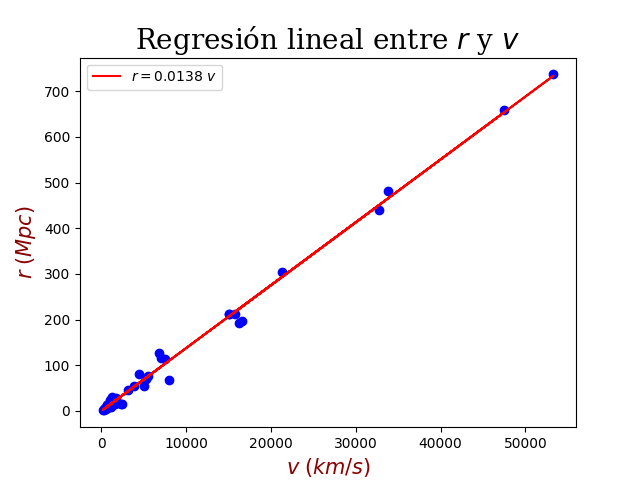
\includegraphics[scale=0.45]{files/plot2}
\end{center}

\vspace{20px}
